\section{Citizens' Avatar}

The feature is described as "As a \gls{guardian} I would like to see the avatars of a \gls{citizen} on the choose citizen screen so that I can quickly identify them." This user story would result in avatars on the \textit{choose citizen} screen, instead of the standard background we can see in \autoref{fig:finalCitizenScreen}.

\begin{figure}[H]
    \begin{center}
        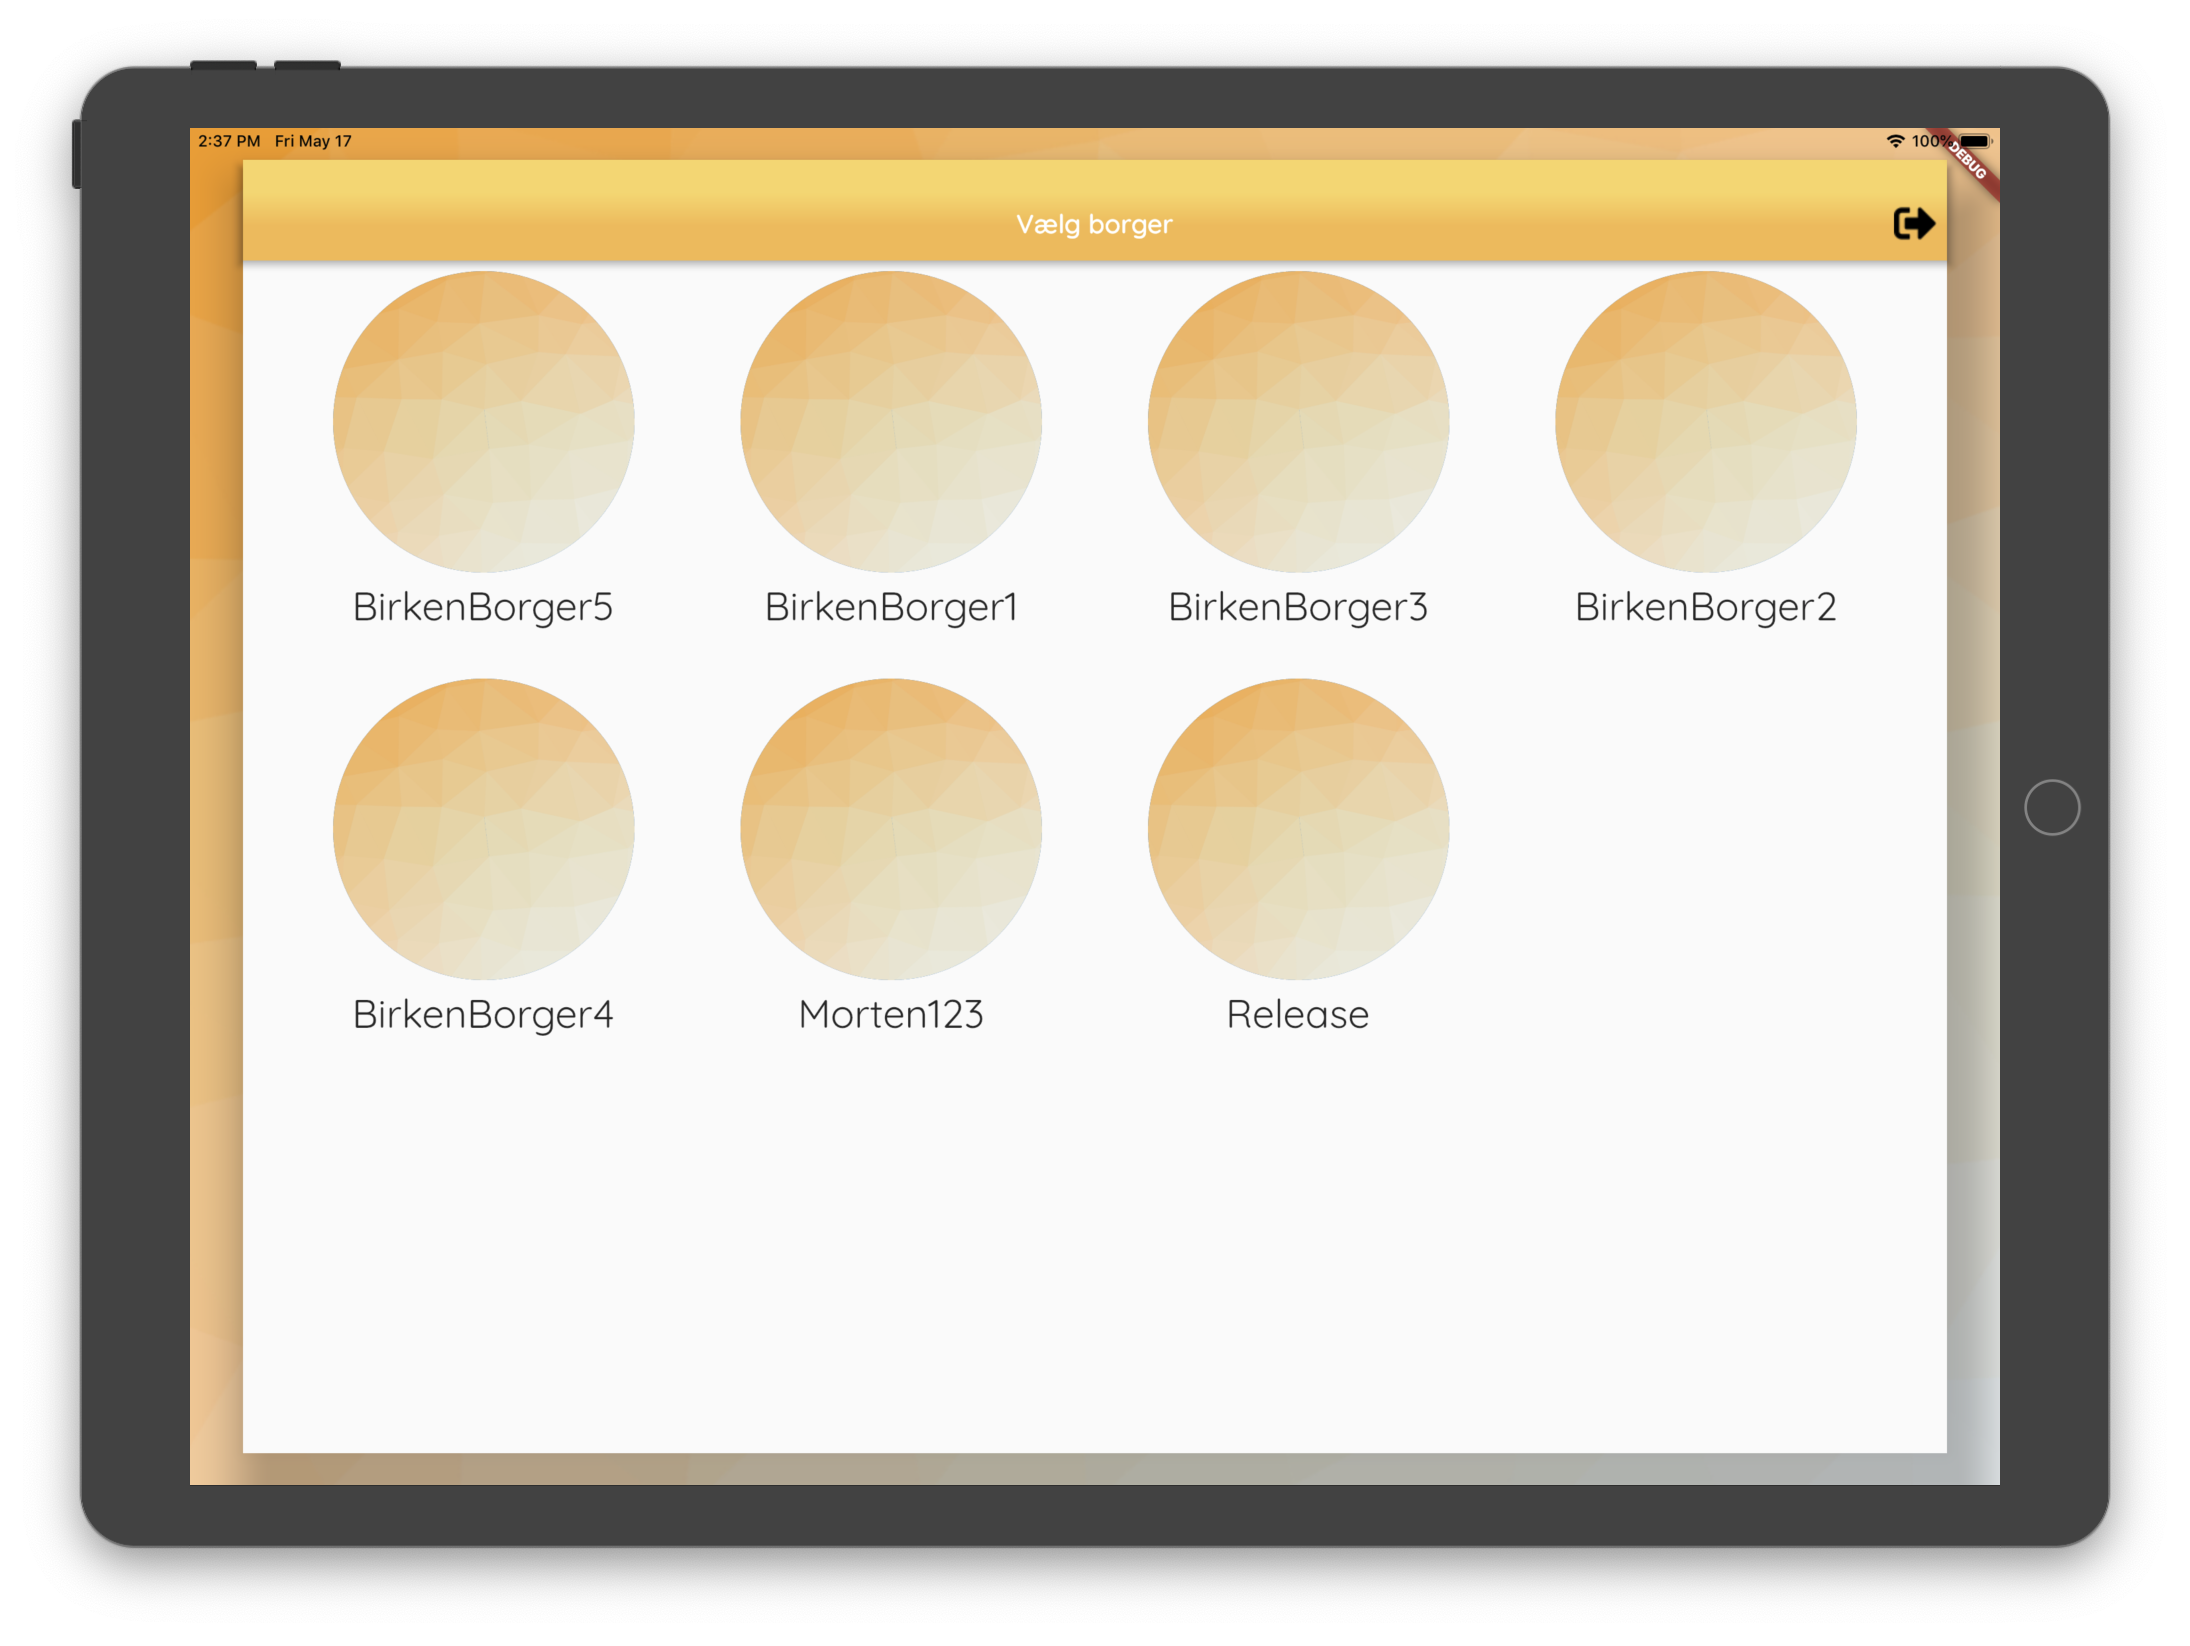
\includegraphics[width=0.95\textwidth]{figures/FinalScreen/chooseCitizenScreen.png}
    \end{center}
    \caption{The \textit{choose citizen} screen}
    \label{fig:finalCitizenScreen}
\end{figure}

We discovered that the location of the standard background was the asset folder. We found that the \gls{fapi} already had a function to retrieve an avatar from a citizen with a given ID.

After we had changed the image source, we found that no \gls{citizen} had an avatar stored. Unfortunately, when we tried to set an avatar for a \gls{citizen}, the \gls{api} would encounter an error when serving it back.

The \gls{POT} estimated that the effort it would take to get the server to deliver the avatars was higher than the importance of the avatars. They told us to stop working on the feature, and therefore, we never completed the user story.